\documentclass[degree=master,tocarialchapter]{thuthesis}
% 选项
%   degree=[bachelor|master|doctor|postdoctor], % 必选,学位类型
%   language=[chinese|english], % 可选(默认:chinese),论文的主要语言
%   secret,                % 可选(默认:关闭),是否有密级
%   tocarialchapter,       % 可选(默认:关闭),章目录中使用黑体(这项表示同时打开下面两项)
%   tocarialchapterentry,  % 可选(默认:关闭),单独控制章标题在目录中使用黑体
%   tocarialchapterpage,   % 可选(默认:关闭),单独控制章页码在目录中使用黑体

% 所有其它可能用到的包都统一放到这里了,可以根据自己的实际添加或者删除。
\usepackage{thuthesis}
\usepackage{codeformat}

% 定义所有的图片文件在 figures 子目录下
\graphicspath{{figures/}}

% 可以在这里修改配置文件中的定义。导言区可以使用中文。
% \def\myname{薛瑞尼}

\begin{document}

%%% 封面部分
\frontmatter
\thusetup{
  %******************************
  % 注意:
  %   1. 配置里面不要出现空行
  %   2. 不需要的配置信息可以删除
  %******************************
  %
  %=====
  % 秘级
  %=====
  % secretlevel={秘密},
  % secretyear={10},
  %
  %=========
  % 中文信息
  %=========
  ctitle={基于BLE Mesh的智能家居平台\\研究报告},
  cdepartment={金苹果锦城第一中学},
  cmajor={计算机科学与技术},
  cauthor={李董睿煊、翟羽佳},
  csupervisor={伍冬莉},
  % 日期自动使用当前时间,若需指定按如下方式修改:
  % cdate={超新星纪元},
  %
  % 博士后专有部分
  % catalognumber     = {分类号},  % 可以留空
  % udc               = {UDC},  % 可以留空
  % id                = {编号},  % 可以留空: id={},
  % cfirstdiscipline  = {计算机科学与技术},  % 流动站(一级学科)名称
  % cseconddiscipline = {系统结构},  % 专 业(二级学科)名称
  % postdoctordate    = {2009 年 7 月——2011 年 7 月},  % 工作完成日期
  % postdocstartdate  = {2009 年 7 月 1 日},  % 研究工作起始时间
  % postdocenddate    = {2011 年 7 月 1 日},  % 研究工作期满时间
  %
  %=========
  % 英文信息
  %=========
  % etitle={An Introduction to \LaTeX{} Thesis Template of Tsinghua University v\version},
  % 这块比较复杂,需要分情况讨论:
  % 1. 学术型硕士
  %    edegree:必须为Master of Arts或Master of Science(注意大小写)
  %             “哲学、文学、历史学、法学、教育学、艺术学门类,公共管理学科
  %              填写Master of Arts,其它填写Master of Science”
  %    emajor:“获得一级学科授权的学科填写一级学科名称,其它填写二级学科名称”
  % 2. 专业型硕士
  %    edegree:“填写专业学位英文名称全称”
  %    emajor:“工程硕士填写工程领域,其它专业学位不填写此项”
  % 3. 学术型博士
  %    edegree:Doctor of Philosophy(注意大小写)
  %    emajor:“获得一级学科授权的学科填写一级学科名称,其它填写二级学科名称”
  % 4. 专业型博士
  %    edegree:“填写专业学位英文名称全称”
  %    emajor:不填写此项
  % edegree={Doctor of Engineering},
  % emajor={Computer Science and Technology},
  % eauthor={Xue Ruini},
  % esupervisor={Professor Zheng Weimin},
  % eassosupervisor={Chen Wenguang},
  % 日期自动生成,若需指定按如下方式修改:
  % edate={December, 2005}
  %
  % 关键词用“英文逗号”分割
  ckeywords={智能家居, BLE Mesh, 插件化, 开放平台},
  % ekeywords={TeX, LaTeX, CJK, template, thesis}
}
\begin{schoollogo}
  \begin{figure}[H]
    \centering
    
\includegraphics{logo.png}
  \end{figure}
\end{schoollogo}
% 定义中英文摘要和关键字
\begin{cabstract}
  本项目主要实现了一个基于BLE Mesh的智能家居平台,分为BLE Mesh节点、网关端、移动端三部分,相较于现有其他智能家居其主要优势是高扩展性、高灵活性、高开放性以及低成本。对于一般用户,降低了将自己整个家庭升级为真正的智能家庭的难度;而对于具有一定技术能力的用户以及爱好者或其他智能家居厂商,则提供了一个开放的平台来更便捷地接入自己的智能设备或控制软件来实现自己的想法。

  本项目的创新点主要有:
  \begin{itemize}
    \item 使用BLE Mesh协议作为节点间通讯的协议,使得节点布置更加方便,不必考虑传统的单对多信号覆盖问题。
    \item 使用低成本的Nordic nRF52832芯片作为BLE Mesh节点,使得用户能够更低成本地使用智能家居。
    \item 具有可选的网关端,使得用户能够更低成本地构建智能家庭系统。
    \item 网关端采用全插件化的方案,使得具有技术能力的用户能够更好、更简单地扩展网关端功能。
    \item 网关端支持Apple HomeKit协议,使得苹果设备用户能用系统原生的“家庭”应用更方便地控制整个智能家庭系统。
    \item 网关端使用高性能的Go语言开发,使得网关端运行更加稳定。
    \item 移动端使用Flutter框架开发,使得在Android/iOS平台中应用体验无太大差异。
  \end{itemize}
\end{cabstract}

% 如果习惯关键字跟在摘要文字后面,可以用直接命令来设置,如下:
% \ckeywords{\TeX, \LaTeX, CJK, 模板, 论文}

% \begin{eabstract}
%    An abstract of a dissertation is a summary and extraction of research work
%    and contributions. Included in an abstract should be description of research
%    topic and research objective, brief introduction to methodology and research
%    process, and summarization of conclusion and contributions of the
%    research. An abstract should be characterized by independence and clarity and
%    carry identical information with the dissertation. It should be such that the
%    general idea and major contributions of the dissertation are conveyed without
%    reading the dissertation.

%    An abstract should be concise and to the point. It is a misunderstanding to
%    make an abstract an outline of the dissertation and words ``the first
%    chapter'', ``the second chapter'' and the like should be avoided in the
%    abstract.

%    Key words are terms used in a dissertation for indexing, reflecting core
%    information of the dissertation. An abstract may contain a maximum of 5 key
%    words, with semi-colons used in between to separate one another.
% \end{eabstract}

% \ekeywords{\TeX, \LaTeX, CJK, template, thesis}

% 如果使用授权说明扫描页,将可选参数中指定为扫描得到的 PDF 文件名,例如:
% \makecover[scan-auth.pdf]
\makecover

%% 目录
\tableofcontents

%% 符号对照表
%\begin{denotation}[3cm]
\item[HPC] 高性能计算 (High Performance Computing)
\item[cluster] 集群
\item[Itanium] 安腾
\item[SMP] 对称多处理
\item[API] 应用程序编程接口
\item[PI] 聚酰亚胺
\item[MPI] 聚酰亚胺模型化合物,N-苯基邻苯酰亚胺
\item[PBI] 聚苯并咪唑
\item[MPBI] 聚苯并咪唑模型化合物,N-苯基苯并咪唑
\item[PY] 聚吡咙
\item[PMDA-BDA]	均苯四酸二酐与联苯四胺合成的聚吡咙薄膜
\item[$\Delta G$] 活化自由能 (Activation Free Energy)
\item[$\chi$] 传输系数 (Transmission Coefficient)
\item[$E$] 能量
\item[$m$] 质量
\item[$c$] 光速
\item[$P$] 概率
\item[$T$] 时间
\item[$v$] 速度
\item[劝学] 君子曰:学不可以已。青,取之于蓝,而青于蓝;冰,水为之,而寒于水。木
  直中绳。輮以为轮,其曲中规。虽有槁暴,不复挺者,輮使之然也。故木受绳则直,金就
  砺则利,君子博学而日参省乎己,则知明而行无过矣。吾尝终日而思矣,不如须臾之所学
  也;吾尝跂而望矣,不如登高之博见也。登高而招,臂非加长也,而见者远;顺风而呼,
  声非加疾也,而闻者彰。假舆马者,非利足也,而致千里;假舟楫者,非能水也,而绝江
  河,君子生非异也,善假于物也。积土成山,风雨兴焉;积水成渊,蛟龙生焉;积善成德,
  而神明自得,圣心备焉。故不积跬步,无以至千里;不积小流,无以成江海。骐骥一跃,
  不能十步;驽马十驾,功在不舍。锲而舍之,朽木不折;锲而不舍,金石可镂。蚓无爪牙
  之利,筋骨之强,上食埃土,下饮黄泉,用心一也。蟹六跪而二螯,非蛇鳝之穴无可寄托
  者,用心躁也。—— 荀况
\end{denotation}



% % 也可以使用 nomencl 宏包:

% \printnomenclature[3cm]

% \nomenclature{HPC}{高性能计算 (High Performance Computing)}
% \nomenclature{cluster}{集群}
% \nomenclature{Itanium}{安腾}
% \nomenclature{SMP}{对称多处理}
% \nomenclature{API}{应用程序编程接口}
% \nomenclature{PI}{聚酰亚胺}
% \nomenclature{MPI}{聚酰亚胺模型化合物,N-苯基邻苯酰亚胺}
% \nomenclature{PBI}{聚苯并咪唑}
% \nomenclature{MPBI}{聚苯并咪唑模型化合物,N-苯基苯并咪唑}
% \nomenclature{PY}{聚吡咙}
% \nomenclature{PMDA-BDA}{均苯四酸二酐与联苯四胺合成的聚吡咙薄膜}
% \nomenclature{$\Delta G$}{活化自由能 (Activation Free Energy)}
% \nomenclature{$\chi$}{传输系数 (Transmission Coefficient)}
% \nomenclature{$E$}{能量}
% \nomenclature{$m$}{质量}
% \nomenclature{$c$}{光速}
% \nomenclature{$P$}{概率}
% \nomenclature{$T$}{时间}
% \nomenclature{$v$}{速度}



%%% 正文部分
\mainmatter
\chapter{引言}

\section{研究背景}
如今,我们正处于一个万物互联的时代。小至智能手表、智能手机,大至铁路运输网、航空运输图,一切都直接或间接连接到了我们的互联网。

在我们的日常生活中,许多灯泡、开关、温湿度传感器前面也加上了“智能”。有了“智能”化的这些物件,意味着我们可以在手机上控制它们、让它们之间按照一定的规则自动调控,更加便利了我们的生活。

但实际上,我们很难能够实现真正意义上的智能:不同的智能设备多来自于不同的智能厂商,而不同厂商又拥有他们独自的控制软件,彼此不互通,导致根本不能实现自动调控;当用户要操控设备时,也要在众多控制App中选择,显得十分繁琐。

\section{研究内容}
本项目主要实现了一个通用的、高扩展性的基于BLE Mesh的智能家居平台,其分为BLE Mesh节点、网关端、移动端三部分。

本项目的BLE Mesh网络可以只由节点组成,并不强制需要网关的参与。本项目节点中采用的Nordic nRF52832芯片也具有低成本的特点,每个节点还可接入多个传感器、继电器等模块,让更多用户有可能将自己整个家庭升级为真正的智能家庭。具有一定技术能力的用户也可根据未来完全开源的PCB、代码等资源自行构建。

本项目的网关端采用了全插件化的方案,用户只需将需要的插件放至网关端插件目录中,就可以接入其他设备以及其他的控制平台,目前本项目已经开发了HomeKit插件来接入到Apple HomeKit。具有一定技术能力的用户也可根据网关端插件API自制插件,以接入自己原有的智能家居硬件或是自己的智能家居控制软件。

本项目的移动端使用Flutter框架开发,具有多平台界面逻辑的一致性,并使用了Material Design,使得界面简洁明了,软件易用性强。
\section{研究难点}
本项目涉及到的方面很多,既涉及到嵌入式设备,又涉及到网络应用开发及移动应用设计。项目的架构设计、流程设计、技术选型、代码的实现、版本管理等都具有一定挑战性。

本项目的BLE Mesh节点,需要考虑到多功能与低功耗之间的平衡,还需要对代码进行优化,以便在相对低性能的嵌入式芯片上正常地运行程序。

本项目的网关端使用了全插件化的方案,在研究过程中需要处处考虑到不同设备间的兼容问题,并且为了方便具有一定技术能力的用户自行开发新插件,还需确保插件API开放的能力足够。

本项目的移动端虽使用了Flutter框架开发,但iOS/Android平台的差异仍要单独考虑,并且调用各平台独有接口的方式变得更加复杂,有时还需要针对各平台编写对应的插件来解决调用独有接口的问题。
\section{创新点}
本项目的创新点主要有以下几点:
\begin{itemize}
    \item 使用BLE Mesh协议作为节点间通讯的协议,使得节点布置更加方便,不必考虑传统的单对多信号覆盖问题。
    \item 使用低成本的Nordic nRF52832芯片作为BLE Mesh节点,使得用户能够更低成本地使用智能家居。
    \item 具有可选的网关端,使得用户能够更低成本地构建智能家庭系统。
    \item 网关端采用全插件化的方案,使得具有技术能力的用户能够更好、更简单地扩展网关端功能。
    \item 网关端支持Apple HomeKit协议,使得苹果设备用户能用系统原生的“家庭”应用更方便地控制整个智能家庭系统。
    \item 网关端使用高性能的Go语言开发,使得网关端运行更加稳定。
    \item 移动端使用Flutter框架开发,使得在Android/iOS平台中应用体验无太大差异。
\end{itemize}
% \chapter{可行性及需求分析}

\section{需求分析}
我们项目的产品要达到以下几点:
  \begin{itemize}
    \item 大范围的覆盖能力;
    \item 对大规模节点设备的检测与控制能力;
    \item 尽可能优化的低功耗能力;
    \item 与目前的智能手机、平板、PC产品兼容;
    \item 工业保准级别的安全性。
  \end{itemize}
\section{可行性分析}
在BLE Mesh技术领域, 在设备端的BLE Mesh节点上, 包括模组的硬件与嵌入式的固件部分, 在性能的研发上, 领先Zigbee很多。

BLE4.0技术具有成本低、低功耗、3ms低延迟、连接距离长等优点,并且目前大部分手机都支持BLE4.0技术,因此用户可以在手机上安装相应的APP,通过APP实现对BLE Mesh网络的控制。\cite{compareblezig} 关闭冗余的可行性及需求分析
\chapter{采用的技术手段}

\section{蓝牙低功耗}
蓝牙低功耗(Bluetooth Low Energy,或称Bluetooth LE、BLE,旧商标Bluetooth Smart)也称蓝牙低能耗、低功耗蓝牙,是蓝牙技术联盟设计和销售的一种个人局域网技术,旨在用于医疗保健、运动健身、信标、安防、家庭娱乐等领域的新兴应用。相较经典蓝牙,低功耗蓝牙旨在保持同等通信范围的同时显著降低功耗和成本。\cite{ble}此外,蓝牙低功耗技术还可在传输过程中采用AES-128-CBC加密,在一定程度上保证了传输过程中的安全性。

本项目使用蓝牙低功耗技术实现多个智能家居节点之间及单个智能家居节点与手机的连接。其低功耗的特点,使得节点只需要一枚纽扣电池即可工作很长时间;传输过程中自动加密的特性也使得整个智能家居平台中的安全性得到了一定的保障。

\section{网状网络}
网状网络(英文:Mesh Network)是一种在网络节点间透过动态路由的方式来进行资料与控制指令的传送。这种网络可以保持每个节点间的连线完整,当网络拓扑中有某节点失效或无法服务时,这种架构允许使用“跳跃”的方式形成新的路由后将讯息送达传输目的地。在网状网络中,所有节点都可与拓扑中所有节点进行连线而形成一个“局域网络”。网状网络与一般网络架构的差异处在于,所有节点可以透过多次跳跃进行数据通信,但它们通常不是移动式装置。网状网络可以视为是一种点对点的架构。移动式点对点网络与网状网络在架构上是非常相似的,只是移动式点对点网络还必须随时更新组态以因应各节点移动的情形。\cite{mesh}

本项目使用网状网络技术增强了智能家居节点布局的灵活性,在部署新节点时只需保证其与现有的任意节点能建立连接即可。移动端也可接入到任意节点,实现从单点控制整个网状网络。

\section{Flutter}
Flutter是一个由谷歌开发的开源移动应用软件开发工具包,用于为Android和iOS开发应用,同时也将是Google Fuchsia下开发应用的主要工具。\cite{flutter}

Flutter的引擎使用C++开发,通过谷歌的Skia图形库提供底层渲染支持,亦提供平台相关的SDK,例如Android和iOS。Flutter框架包含了两套符合特定设计语言的组件。 称作Material Design的组件实现的是同名的谷歌设计语言,称作Cupertino的组件模仿了苹果iOS的设计Flutter是通过组织、创建不同的组件完成用户界面设计的。 在Flutter中,一个组件代表用户界面中不可变的一部分;包括文本、多边形以及动画在内的所有图形都是用组件创建的。复杂的组件由简单的组件结合而成。基础库由Dart编写,提供了用Flutter构建应用所需的基本的类和函数,例如与引擎通讯的API。\cite{flutter}

我们利用Flutter一次开发多平台使用来起到多平台UI及功能的统一性。Flutter的热重载帮助我们快捷方便的试验、重构UI、添加特性和修复bug。在仿真器、模拟器和iOS、Android硬件上快速重载,而不会丢失状态。使用Flutter内置美丽的Material Design和Cupertino(iOS风格)widget、丰富的motion API、平滑而自然的滑动效果和平台感知,为用户带来全新体验。使用Flutter的现代、响应式框架,和一系列基础widget,轻松构建用户界面。使用功能强大且灵活的API(针对2D、动画、手势、效果等)解决艰难的UI挑战。\cite{quickdev}

\chapter{基于BLE Mesh的智能家居平台功能设计}

\section{架构设计}
本项目主要分为三个部分:BLE Mesh节点,网关端及移动端(如图~\ref{fig:arch_basic})。

BLE Mesh节点主要实现传感器、继电器、灯泡等设备的接入,并且节点间可自动建立BLE协议下的Mesh网络,使得用户即使不使用网关也能用移动端软件连接至Mesh网络控制所有节点。

网关端主要实现设备层与管理应用层的连接。采用插件化的方案,使得有能力的爱好者或其他智能设备厂商,可以自己根据本项目简单的API来制作插件接入本平台;也便于接入到其他的管理平台,例如Apple HomeKit、Google Home等,让用户不需要下载其他程序就能管理网关下的所有设备。

移动端主要实现控制Mesh网络或网关下的设备、添加自动化的功能。
\begin{figure}[H]
    \centering
    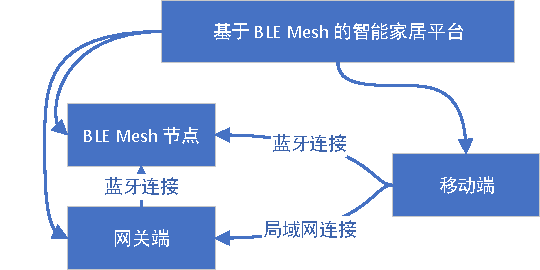
\includegraphics{arch_basic.pdf}
    \caption{基于BLE Mesh的智能家居平台基本架构图}
    \label{fig:arch_basic}
\end{figure}

\section{BLE Mesh节点}
\label{design:blemeshnode}
BLE Mesh节点不同于一般智能家居设备,它们之间通过另一个BLE Mesh分发节点或手机分发配置后构成网状网络,之后所有数据就可通过其他节点转发至目标设备(如图~\ref{fig:arch_mesh})。

每个节点均可接入多个模块,例如继电器、开关、传感器等。不需要每个模块都单独配一套蓝牙通讯装置,节约了成本也节约了频段资源。

网关或移动端设备也可以通过任一节点代理入Mesh网络,之后便可以访问所有的节点及其连接的模块。
\begin{figure}[H]
    \centering
    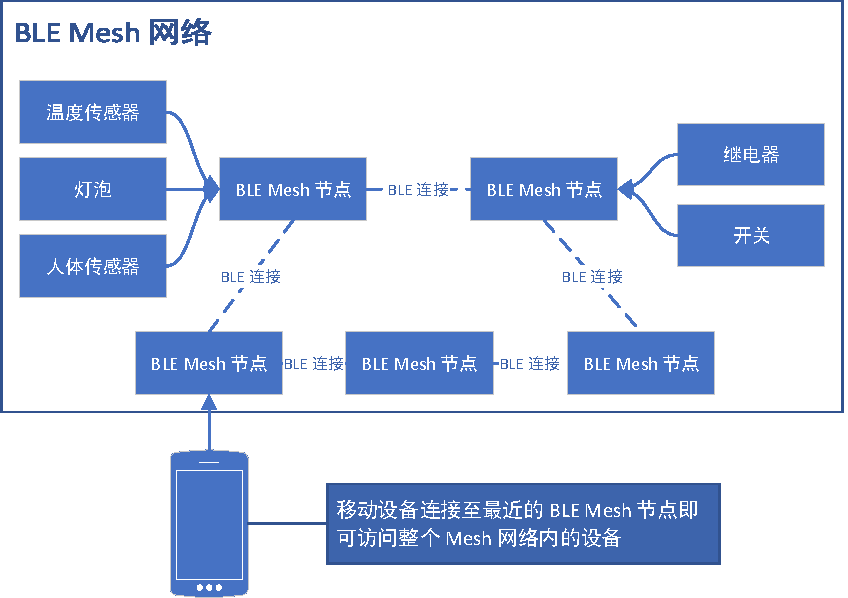
\includegraphics{arch_mesh.pdf}
    \caption{基于BLE Mesh的智能家居平台BLE Mesh网络架构图}
    \label{fig:arch_mesh}
\end{figure}

\section{网关端}
网关端实现了设备层与管理应用层的连接,即将不同的智能设备(如~\ref{design:blemeshnode}~章所提到的BLE Mesh节点等)与不同的管理平台(如~\ref{design:mobile}~章所提到的基于BLE Mesh的智能家居平台移动端、Apple HomeKit等)相连接。

网关端还创新性地采用了插件化的方案(如图~\ref{fig:arch_gateway}),使得爱好者或智能家居厂商可自行按照网关端插件API编写对应插件,让家中所有的智能设备最终能在一个平台上进行管理。目前本项目已开发的插件有BLE Mesh插件(用于连接BLE Mesh节点)、本项目移动端所使用的WebSocket插件(将设备以WebSocket的方式暴露到内网便于移动端连接)以及Apple HomeKit插件(将设备以符合Apple HomeKit方式暴露到内网便于苹果设备上的“家庭”应用连接)。
\begin{figure}[H]
    \centering
    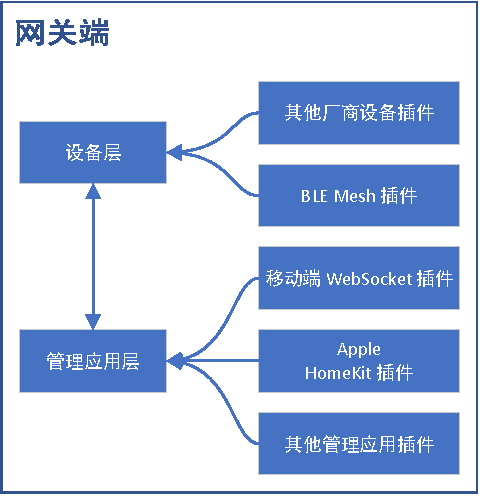
\includegraphics{arch_gateway.pdf}
    \caption{基于BLE Mesh的智能家居平台网关端架构图}
    \label{fig:arch_gateway}
\end{figure}

\section{移动端}
\label{design:mobile}
移动端包含了UI层、设备层及自动化层(如图~\ref{fig:arch_mobile})。UI层支持用户查看所有设备的状态、控制所有设备及添加自动化流程。设备层支持通过单个BLE Mesh节点代理入网的方式及通过连接至网关端WebSocket插件的方式访问整个智能家居网络。而自动化层支持用户在本机执行自动化流程或将自动化流程提交到网关。
\begin{figure}[H]
    \centering
    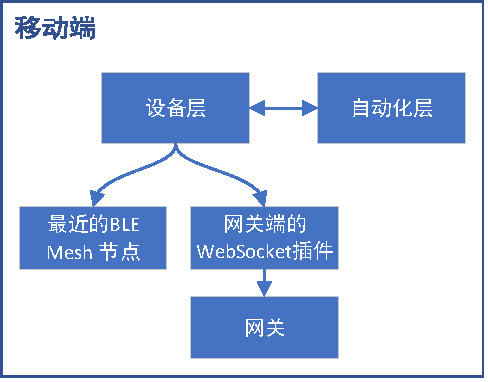
\includegraphics{arch_mobile.pdf}
    \caption{基于BLE Mesh的智能家居平台移动端架构图}
    \label{fig:arch_mobile}
\end{figure}

\chapter{基于BLE Mesh的智能家居平台实现}
\section{开发语言的选择}
现今,市面上有许多开发语言可供选择,它们各自有各自的优点,如C/C++语言执行速度快,程序占用空间小;Go语言代码简洁,执行速度快;Dart语言易于编写,使用Flutter框架后还可实现一套代码就能编译出iOS/Android端的App。

对于本项目的BLE Mesh节点而言,其性能不高且存储空间狭小,并且需使用Nordic芯片厂商所提供的nRF5 SDK for Mesh,因此选择了C语言作为开发语言。

对于本项目的网关端而言,其性能充足但需要高扩展性且逻辑复杂,为了开发方便,因此选择了Go语言作为开发语言。

对于本项目的移动端而言,需要同时支持Android与iOS系统,为了界面逻辑统一,因此选择了Dart语言与Flutter框架作为开发语言。

\section{集成开发环境的选择}
在BLE Mesh节点开发上,目前针对嵌入式开发并支持C语言主要是SEGGER Embedded Studio及Keil,SEGGER Embedded Studio相较于Keil更加易用,并且能很好地兼容nRF5 SDK for Mesh,因此选择了SEGGER Embedded Studio作为BLE Mesh节点的集成开发环境。

在网关端开发上,目前针对Go语言的集成开发环境主要有GoLand与VS Code,但GoLand功能更为强大,能很好地进行调试以及包管理,因此选择了GoLand作为网关端的集成开发环境。

在移动端开发上,目前Google推荐使用Android Studio进行Dart+Flutter的开发,因此选择了Android Studio作为移动端的集成开发环境。

\section{逻辑部分的实现}
\subsection{BLE Mesh节点}
BLE Mesh节点主要分为两个角色,一个是Server,一个是Provisioner。Server作为连接继电器、传感器等模块的角色,而Provisioner则负责给未配置的Server节点发放BLE Mesh网络配置。本项目采用Nordic的nRF5 SDK for Mesh来处理BLE Mesh协议栈的底层调用。

\subsubsection{Server}
Server节点在上电后初始化BLE、Mesh协议栈及其他参数,开始发送Unprovisioned Node Beacon广播信息,等待Provisioner分发配置,配网成功后注册GATT服务与传感器服务,以便移动端或网关端BLE Mesh插件通过此节点代理入网,并允许其他节点访问它的模块。

\begin{figure}[H]
    \centering
    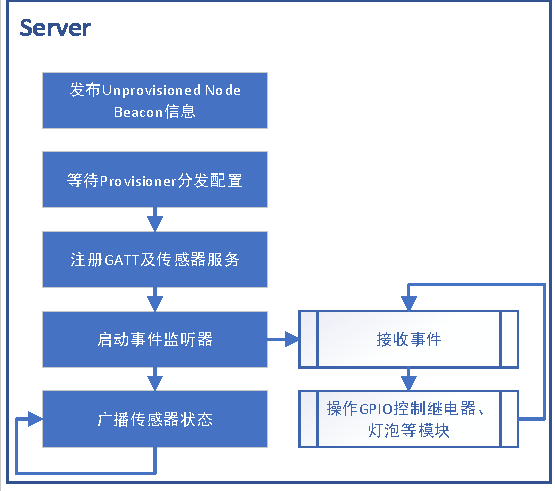
\includegraphics{flowchart_mesh_server.pdf}
    \caption{基于BLE Mesh的智能家居平台BLE Mesh Server节点流程图}
    \label{fig:flowchart_mesh_server}
\end{figure}

\begin{figure}[H]
    \centering
    \begin{lstlisting}[language=C]
    ble_stack_init();
    gap_params_init();
    conn_params_init();
    mesh_init();
    //初始化蓝牙协议栈、GATT参数、传感器参数、Mesh协议栈
    if (!m_device_provisioned){
        //设备未配网
        static const uint8_t static_auth_data[NRF_MESH_KEY_SIZE] = STATIC_AUTH_DATA;
        //配置OOB预认证密钥
        mesh_provisionee_start_params_t prov_start_params = {
            .p_static_data    = static_auth_data,
            .prov_complete_cb = provisioning_complete_cb,
            .prov_device_identification_start_cb = device_identification_start_cb,
            .prov_device_identification_stop_cb = NULL,
            .prov_abort_cb = provisioning_aborted_cb,
            .p_device_uri = EX_URI_LS_SERVER
        };
        mesh_provisionee_prov_start(&prov_start_params);
        //启动Provisionee过程,等待配网结束
    }
    mesh_app_uuid_print(nrf_mesh_configure_device_uuid_get());
    //输出配网后分配到的设备UUID以供调试使用
    mesh_stack_start();
    //启动Mesh协议栈
    \end{lstlisting}
    \caption{基于BLE Mesh的智能家居平台BLE Mesh Server节点关键代码}
    \label{fig:code_mesh_server}
\end{figure}

\subsubsection{Provisioner}
Provisioner节点上电后初始化BLE、Mesh协议栈,从,等待接收Server节点发送的Unprovisioned Node Beacon广播,与Server节点协商通信使用的加密算法,交换非对称加密算法的公钥,之后验证Server节点的OOB预配置密钥,验证成功后向Server节点发送加密后配网信息,之后再重新开始接收未配置节点对广播,为每一个未配置的Server节点进行配网操作。

\begin{figure}[H]
    \centering
    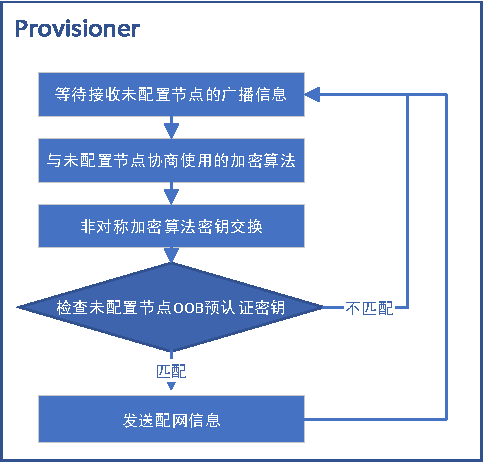
\includegraphics{flowchart_mesh_provisioner.pdf}
    \caption{基于BLE Mesh的智能家居平台BLE Mesh Provisioner节点流程图}
    \label{fig:flowchart_mesh_provisioner}
\end{figure}

\begin{figure}[H]
    \centering
    \begin{lstlisting}[language=C]
    static void startprovision(){
        static const char * uri_list[1];
        uri_list[0] = server_uri_index_select(m_nw_state.p_client_uri);
        //设置可用的配网器为自己
        prov_helper_provision_next_device(PROVISIONER_RETRY_COUNT, m_nw_state.next_device_address, uri_list, ARRAY_SIZE(uri_list));
        //开始对未配网列表中的首个设备进行配网
        prov_helper_scan_start();
        //配网完成,继续扫描未配网设备
    }

    static void start(){
        //程序入口
        ble_stack_init();
        mesh_init();
        //初始化蓝牙协议栈、Mesh协议栈
        nrf_mesh_enable();
        //启动Mesh协议栈
        while(true){
            startprovision();
            //进行配网操作
        }
    }
    \end{lstlisting}
    \caption{基于BLE Mesh的智能家居平台BLE Mesh Provisioner节点关键代码}
    \label{fig:code_mesh_provisioner}
\end{figure}

\subsection{网关端}
\subsubsection{主程序}
网关端在启动后扫描plugin/accessory和plugin/consumer目录下的插件,并一一加载设备层插件,获取所有节点列表后,再一一加载管理应用层插件,以协程的方式并行启动每个插件的工作函数,最后阻塞主协程(如图~\ref{fig:flowchart_gateway}~,图~\ref{fig:code_gateway})。

网关端还使用了brutella/hc项目中的智能家居结构模型(如图~\ref{fig:hc_structure}),即将每个节点看作Accessory(配件),将节点上所接入的模块模块看作Service(服务),将每个模块能提供或设定的数据看作Characteristic(特性)。

\begin{figure}[H]
    \centering
    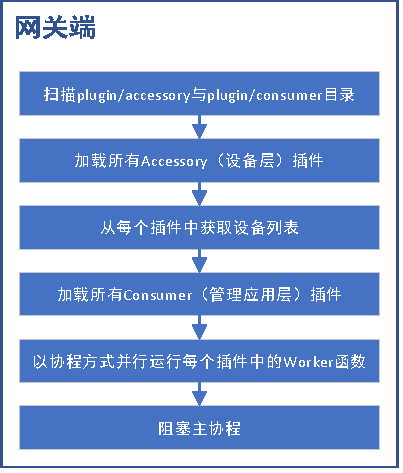
\includegraphics{flowchart_gateway.pdf}
    \caption{基于BLE Mesh的智能家居平台网关端流程图}
    \label{fig:flowchart_gateway}
\end{figure}

\begin{figure}[H]
    \centering
    \begin{lstlisting}[language=Go]
    func LoadAccessoryPlugin(){
        accpluginfiles,_:=ioutil.ReadDir(AccPluginDir)
        for _, f := range accpluginfiles{
            plug, err := plugin.Open(AccPluginDir+f.Name())
            sym, err := plug.Lookup("Plugin")
            accplugin := sym.(AccessoryPlugin)
            AccessoryPluginList = append(AccessoryPluginList, accplugin)
        }
    }
    func LoadConsumerPlugin(){
        conpluginfiles,_:=ioutil.ReadDir(ConPluginDir)
        for _, f := range conpluginfiles{
            plug, err := plugin.Open(ConPluginDir+f.Name())
            sym, err := plug.Lookup("Plugin")
            conplugin := sym.(ConsumerPlugin)
            ConsumerPluginList = append(ConsumerPluginList, conplugin)
        }
    }
    func InitAccessoryPlugin(){
        for _, accplugin := range AccessoryPluginList{
            accplugin.Init(Shutdown)
            AccessoryList = append(AccessoryList,accplugin.GetAccessoryList()...)
        }
    }
    func InitConsumerPlugin(){
	    for _, conplugin := range ConsumerPluginList{
	    	conplugin.Init(AccessoryList)
	    }
    }
    func main(){
        LoadAccessoryPlugin()
        LoadConsumerPlugin()
        InitAccessoryPlugin()
        InitConsumerPlugin()
        for _, accplugin := range AccessoryPluginList{
            go accplugin.Worker()
        }
        for _, conplugin := range ConsumerPluginList{
            go conplugin.Worker()
        }
        for{
            c := ""
            _, _ = fmt.Scanln(&c)
            if c == "stop"{Shutdown()}
        }
    }
    \end{lstlisting}
    \caption{基于BLE Mesh的智能家居平台网关端关键代码}
    \label{fig:code_gateway}
\end{figure}

\begin{figure}[H]
    \centering
    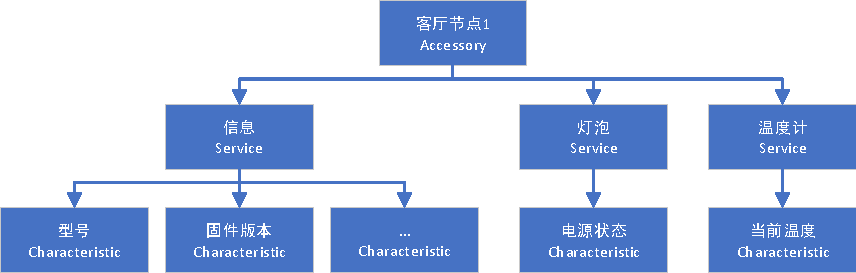
\includegraphics{hc_structure.pdf}
    \caption{brutella/hc项目中的智能家居结构模型示意图}
    \label{fig:hc_structure}
\end{figure}

\subsubsection{BLE Mesh插件}
BLE Mesh插件在启动后连接最近的BLE Mesh节点,然后获取Mesh网络中所有的节点及其服务,之后将信息转化为Accessory对象,用Characteristic中的闭包来处理更新事件,

\begin{figure}[H]
    \centering
    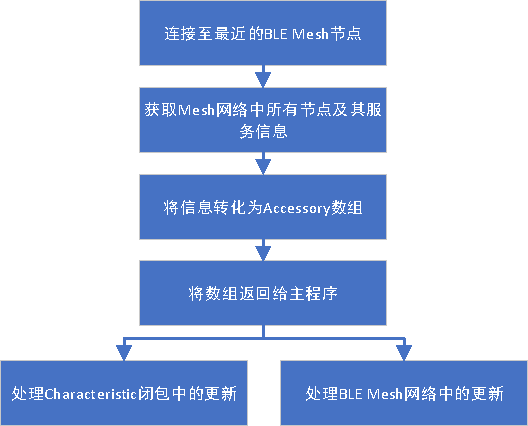
\includegraphics{flowchart_gateway_plugin_blemesh.pdf}
    \caption{基于BLE Mesh的智能家居平台网关端BLE Mesh插件流程图}
    \label{fig:flowchart_gateway_plugin_blemesh}
\end{figure}

\begin{figure}[H]
    \centering
    \begin{lstlisting}[language=Go]
    func (p *AccPlugin) Init(){
        p.Meshnodes = ConnectToMeshNetwork()
        meshaccessories := MeshNode2Accessory(p.Meshnodes)
        for accid, acc := range meshaccessories{
            for _, srv := range acc.Services{
                for _, cha := range srv.Characteristics{
                    cha.OnValueUpdate(func(c *characteristic.Characteristic, newValue, oldValue interface{}){
                        meshnodes[accid].notify(c.Type,newValue)
                    })
                }
            }
        }
        p.AccessoryList = meshaccessories
    }
    func (p *AccPlugin) GetAccessoryList() []*accessory.Accessory{
	    return p.AccessoryList
    }
    func (p *AccPlugin) Worker(){
        for _, meshnode := range p.Meshnodes{
            meshnode.AddListener(func(type String,value interface{}){
                meshnode.Accessory.Change(type, value)
            })
        }
    }
    \end{lstlisting}
    \caption{基于BLE Mesh的智能家居平台网关端BLE Mesh插件关键代码}
    \label{fig:code_gateway_plugin_blemesh}
\end{figure}

\subsubsection{WebSocket插件}
WebSocket插件在初始化时对Accessory ID和每个Accessory下的Characteristic重新建索,并启动WebSocket服务,处理更新请求以及在任何Characteristic值更新时向所有客户端发送通知。

\begin{figure}[H]
    \centering
    \begin{lstlisting}[language=Go]
    func (p *ConPlugin) Init(list []*accessory.Accessory) {
        p.AccessoryList = list
        for id, acc := range p.AccessoryList {
		for _, srv := range acc.Services {
			for _, cha := range srv.Characteristics {
				p.Cmap[acc.ID][cha.ID] = cha
				func(accid int64) {
					cha.OnValueUpdate(func(c *characteristic.Characteristic, newValue, oldValue interface{}) {
						for _, conn := range Plugin.WebSocketList {
							_ = conn.WriteJSON(models.Response{
								Type: "update",
								Value: models.UpdateReq{
									Aid:   accid,
									Cid:   c.ID,
									Value: newValue,
								},
							})
						}
					})
				}(int64(id)+2)
			}
		}
        }
    }
    func (p *ConPlugin) Worker() {
	    http.HandleFunc("/ws", func(w http.ResponseWriter, r *http.Request) {
            c, err := upgrader.Upgrade(w, r, nil)
            Plugin.WebSocketList = append(Plugin.WebSocketList, c)
            for {
                _, str, err := c.ReadMessage()
                err = json.Unmarshal(str, &req)
                switch req.Command {
                    case "getaccessorylist":
                        res.Value = Plugin.AccessoryList
                        break
                    case "update":
                        umap := req.Value.(map[string]interface{})
                        var updateReq models.UpdateReq
                        err = mapstructure.Decode(umap, &updateReq)
                        Plugin.Cmap[updateReq.Aid][updateReq.Cid].UpdateValue(updateReq.Value)
                }
                c.WriteJSON(res)
            })
	    log.Fatal(http.ListenAndServe(*addr, nil))
    }
    \end{lstlisting}
    \caption{基于BLE Mesh的智能家居平台网关端WebSocket插件关键代码}
    \label{fig:code_gateway_plugin_websocket}
\end{figure}

\subsubsection{HomeKit插件}
HomeKit插件主要调用brutella/hc项目中内置的HomeKit服务端,启动后先生成一个随机配对密钥,再建立一个HomeKit Bridge来作为HomeKit中桥的角色,并将其他的节点挂载到HomeKit Bridge下,最后启动HomeKit服务端来广播HomeKit Bridge。

\begin{figure}[H]
    \centering
    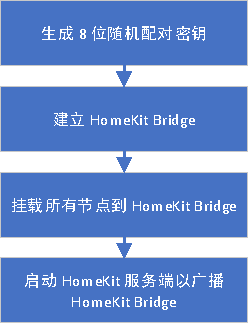
\includegraphics{flowchart_gateway_plugin_homekit.pdf}
    \caption{基于BLE Mesh的智能家居平台网关端HomeKit插件流程图}
    \label{fig:flowchart_gateway_plugin_homekit}
\end{figure}

\begin{figure}[H]
    \centering
    \begin{lstlisting}[language=Go]
    func (p *ConPlugin) Init(list []*accessory.Accessory){
        rand.Seed(time.Now().UnixNano())
        p.Name = "HomeKit (Non-Commercial)"
        p.AccessoryList = list
        p.Bridge = accessory.NewBridge(accessory.Info{
            Name:             "BLESmartHome HomeKit Bridge",
            SerialNumber:     "Bridge_001",
            Manufacturer:     "BLESmartHome",
            Model:            "Plugin_HomeKit",
            FirmwareRevision: "0.0.1",
        })
        p.Config = hc.Config{
            StoragePath: "./plugin/consumer/homekit/",
            Pin:         fmt.Sprintf("%08d",rand.Int()%1e8),
        }
    }
    func (p *ConPlugin) Worker(){
	    t, err := hc.NewIPTransport(p.Config,p.Bridge.Accessory,p.AccessoryList...)
	    p.StopIPTransPort = func() {
	    	t.Stop()
        }
	    fmt.Println("HomeKit Pairing Pin: "+p.Config.Pin)
	    t.Start()
    }
    \end{lstlisting}
    \caption{基于BLE Mesh的智能家居平台网关端HomeKit插件关键代码}
    \label{fig:code_gateway_plugin_homekit}
\end{figure}

\subsection{移动端}

\subsubsection{连接设备}
移动端在用户点击连接设备后,可选择通过蓝牙连接以及通过WLAN连接。

点击通过蓝牙连接,进入蓝牙扫描状态,搜索附近的蓝牙Mesh节点,弹出列表让用户选择后连接,即可通过单一节点代理入网,控制整个网络中的节点及所连接的模块。

点击通过WLAN连接,进入局域网扫描状态,搜索整个网络中已启用WebSocket插件的网关端,弹出列表让用户选择后连接,即可访问网关设备层中的所有节点及所连接的模块。

\begin{figure}[H]
    \centering
    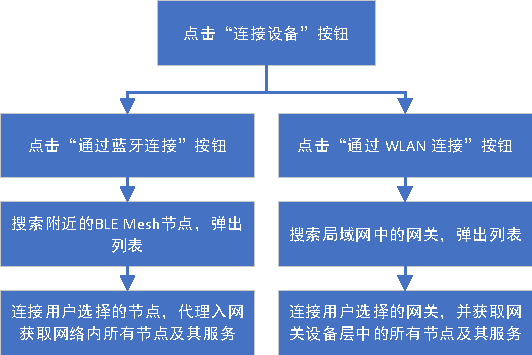
\includegraphics{flowchart_mobile_connect.pdf}
    \caption{基于BLE Mesh的智能家居平台移动端连接设备流程图}
    \label{fig:flowchart_mobile_connect}
\end{figure}

\begin{figure}[H]
    \centering
    \begin{lstlisting}[language=Java]
    BluetoothAdd() {
        meshnodes = scanMeshNodes();
        for(int i=0;i<meshnodes.length;i++){
          meshnodewidgets.add(Card(child: ListTile(onTap: (){
            connectmeshnode(meshnodes[i]);
          },leading: Icon(Icons.bluetooth),title: Text(meshnodes[i].name))));
        }
        showModalBottomSheet(context:this.context,builder:(BuildContext context) {
          return new ListView(children: <Widget>[
            Padding(padding:EdgeInsets.all(20),child:Text("选择 BLE Mesh 节点",textAlign: TextAlign.left,
              style: TextStyle(fontWeight: FontWeight.bold,fontSize: 20),)),
            ]+meshnodewidgets);
        });
    }
    \end{lstlisting}
    \caption{基于BLE Mesh的智能家居平台移动端通过蓝牙连接关键代码}
    \label{fig:code_mobile_connect_ble}
\end{figure}

\begin{figure}[H]
    \centering
    \begin{lstlisting}[language=Java]
    IPAdd() {
        ipnodes = scanIPNodes();
        for(int i=0;i<ipnodes.length;i++){
          ipnodewidgets.add(Card(child: ListTile(onTap: (){
            connectipnode(ipnodes[i]);
          },leading: Icon(Icons.router),title: Text(ipnodes[i].name),subtitle: Text(ipnodes[i].address))));
        }
        showModalBottomSheet(context:this.context,builder:(BuildContext context) {
          return new ListView(children: <Widget>[
            Padding(padding:EdgeInsets.all(20),child:Text("选择网关",textAlign: TextAlign.left,
              style: TextStyle(fontWeight: FontWeight.bold,fontSize: 20),)),
            ]+ipnodewidgets);
        });
    }
    \end{lstlisting}
    \caption{基于BLE Mesh的智能家居平台移动端通过WLAN连接关键代码}
    \label{fig:code_mobile_connect_wlan}
\end{figure}

\subsubsection{控制配件}
在配件列表中,点击可控制的服务后,进行电源状态的切换或弹出其他可调整项,之后将更新发送至连接的BLE Mesh节点或网关端,完成配件的控制。

\begin{figure}[H]
    \centering
    \begin{lstlisting}[language=Java]
    case SERVICE_LIGHTBULB:
        Characteristic c = srv.getCharacteristic(CHAR_ON);
        srv.name = "灯泡";
        value = dynamictoT<bool>(c.value)?"开":"关";
        icon = Icons.lightbulb_outline;
        onclick = (){
            c.value = !dynamictoT<bool>(c.value);
            if(srv.ble){
                bleupdate(srv.aid,c.cid);
            }else{
                wlanupdate(srv.aid,c.cid);
            }
        }
    \end{lstlisting}
    \caption{基于BLE Mesh的智能家居平台移动端控制灯泡服务关键代码}
    \label{fig:code_mobile_control_lightbulb}
\end{figure}

\subsubsection{自动化}
在自动化列表中,点击添加自动化按钮后,弹出选择触发服务菜单,选择用于触发的服务后,进入对应服务的条件界面,设置条件后点击下一步弹出选择操作服务菜单,进入对应服务的操作界面,设置操作后点击完成即添加完成。

\begin{figure}[H]
    \centering
    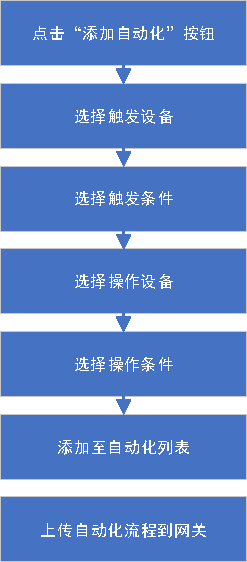
\includegraphics{flowchart_mobile_add_automation.pdf}
    \caption{基于BLE Mesh的智能家居平台移动端添加自动化流程图}
    \label{fig:flowchart_mobile_connect}
\end{figure}

\begin{figure}[H]
    \centering
    \begin{lstlisting}[language=Java]
    AddAutomation(){
        automation = new Automation();
        automation.trigger = gettriggerfrommodal();
        automation.when = getwhenfrommodal();
        automation.opservice = getopsrvfrommodal();
        automation.op = getopfrommodal();
        wlanaddautomation(automation);
        automationlist.add(automation);
    }
    \end{lstlisting}
    \caption{基于BLE Mesh的智能家居平台移动端添加自动化关键代码}
    \label{fig:code_mobile_add_automation}
\end{figure}
\chapter{基于BLE Mesh的智能家居平台测试}
内容

\section{功能测试}
内容

\section{稳定性测试}
内容



%%% 其它部分
%\backmatter

%% 本科生要这几个索引,研究生不要。选择性留下。
% 插图索引
%\listoffigures
% 表格索引
%\listoftables
% 公式索引
%\listofequations


%% 参考文献
% 注意:至少需要引用一篇参考文献,否则下面两行可能引起编译错误。
% 如果不需要参考文献,请将下面两行删除或注释掉。
\bibliographystyle{thuthesis-numeric}      % 顺序编码制
% \bibliographystyle{thuthesis-author-year}  % 著者-出版年制
% \bibliographystyle{thuthesis-bachelor}     % 本科生参考文献的著录格式
\bibliography{ref/refs}


%% 致谢
%% 如果使用声明扫描页,将可选参数指定为扫描后的 PDF 文件名,例如:
% \begin{acknowledgement}[scan-statement.pdf]
\begin{acknowledgement}
  衷心感谢导师 xxx 教授和物理系 xxx 副教授对本人的精心指导。他们的言传身教将使
  我终生受益。

  在美国麻省理工学院化学系进行九个月的合作研究期间,承蒙 xxx 教授热心指导与帮助,不
  胜感激。感谢 xx 实验室主任 xx 教授,以及实验室全体老师和同学们的热情帮助和支
  持!本课题承蒙国家自然科学基金资助,特此致谢。

  感谢 \LaTeX 和 \thuthesis\cite{thuthesis},帮我节省了不少时间。
\end{acknowledgement}


%% 附录
%\begin{appendix}
%\chapter{外文资料原文}
\label{cha:engorg}

\title{The title of the English paper}

\textbf{Abstract:} As one of the most widely used techniques in operations
research, \emph{ mathematical programming} is defined as a means of maximizing a
quantity known as \emph{bjective function}, subject to a set of constraints
represented by equations and inequalities. Some known subtopics of mathematical
programming are linear programming, nonlinear programming, multiobjective
programming, goal programming, dynamic programming, and multilevel
programming$^{[1]}$.

It is impossible to cover in a single chapter every concept of mathematical
programming. This chapter introduces only the basic concepts and techniques of
mathematical programming such that readers gain an understanding of them
throughout the book$^{[2,3]}$.


\section{Single-Objective Programming}
The general form of single-objective programming (SOP) is written
as follows,
\begin{equation*} % 如果附录中的公式不想让它出现在公式索引中,那就请
                             % 用 equation*
\left\{\begin{array}{l}
\max \,\,f(x)\\[0.1 cm]
\mbox{subject to:} \\ [0.1 cm]
\qquad g_j(x)\le 0,\quad j=1,2,\cdots,p
\end{array}\right.
\end{equation*}
which maximizes a real-valued function $f$ of
$x=(x_1,x_2,\cdots,x_n)$ subject to a set of constraints.

\newcommand\Real{\mathbf{R}}
\newtheorem{mpdef}{Definition}[chapter]
\begin{mpdef}
In SOP, we call $x$ a decision vector, and
$x_1,x_2,\cdots,x_n$ decision variables. The function
$f$ is called the objective function. The set
\begin{equation*}
S=\left\{x\in\Real^n\bigm|g_j(x)\le 0,\,j=1,2,\cdots,p\right\}
\end{equation*}
is called the feasible set. An element $x$ in $S$ is called a
feasible solution.
\end{mpdef}

\newtheorem{mpdefop}[mpdef]{Definition}
\begin{mpdefop}
A feasible solution $x^*$ is called the optimal
solution of SOP if and only if
\begin{equation}
f(x^*)\ge f(x)
\end{equation}
for any feasible solution $x$.
\end{mpdefop}

One of the outstanding contributions to mathematical programming was known as
the Kuhn-Tucker conditions\ref{eq:ktc}. In order to introduce them, let us give
some definitions. An inequality constraint $g_j(x)\le 0$ is said to be active at
a point $x^*$ if $g_j(x^*)=0$. A point $x^*$ satisfying $g_j(x^*)\le 0$ is said
to be regular if the gradient vectors $\nabla g_j(x)$ of all active constraints
are linearly independent.

Let $x^*$ be a regular point of the constraints of SOP and assume that all the
functions $f(x)$ and $g_j(x),j=1,2,\cdots,p$ are differentiable. If $x^*$ is a
local optimal solution, then there exist Lagrange multipliers
$\lambda_j,j=1,2,\cdots,p$ such that the following Kuhn-Tucker conditions hold,
\begin{equation}
\label{eq:ktc}
\left\{\begin{array}{l}
    \nabla f(x^*)-\sum\limits_{j=1}^p\lambda_j\nabla g_j(x^*)=0\\[0.3cm]
    \lambda_jg_j(x^*)=0,\quad j=1,2,\cdots,p\\[0.2cm]
    \lambda_j\ge 0,\quad j=1,2,\cdots,p.
\end{array}\right.
\end{equation}
If all the functions $f(x)$ and $g_j(x),j=1,2,\cdots,p$ are convex and
differentiable, and the point $x^*$ satisfies the Kuhn-Tucker conditions
(\ref{eq:ktc}), then it has been proved that the point $x^*$ is a global optimal
solution of SOP.

\subsection{Linear Programming}
\label{sec:lp}

If the functions $f(x),g_j(x),j=1,2,\cdots,p$ are all linear, then SOP is called
a {\em linear programming}.

The feasible set of linear is always convex. A point $x$ is called an extreme
point of convex set $S$ if $x\in S$ and $x$ cannot be expressed as a convex
combination of two points in $S$. It has been shown that the optimal solution to
linear programming corresponds to an extreme point of its feasible set provided
that the feasible set $S$ is bounded. This fact is the basis of the {\em simplex
  algorithm} which was developed by Dantzig as a very efficient method for
solving linear programming.
\begin{table}[ht]
\centering
  \centering
  \caption*{Table~1\hskip1em This is an example for manually numbered table, which
    would not appear in the list of tables}
  \label{tab:badtabular2}
  \begin{tabular}[c]{|m{1.5cm}|c|c|c|c|c|c|}\hline
    \multicolumn{2}{|c|}{Network Topology} & \# of nodes &
    \multicolumn{3}{c|}{\# of clients} & Server \\\hline
    GT-ITM & Waxman Transit-Stub & 600 &
    \multirow{2}{2em}{2\%}&
    \multirow{2}{2em}{10\%}&
    \multirow{2}{2em}{50\%}&
    \multirow{2}{1.2in}{Max. Connectivity}\\\cline{1-3}
    \multicolumn{2}{|c|}{Inet-2.1} & 6000 & & & &\\\hline
    \multirow{2}{1.5cm}{Xue} & Rui  & Ni &\multicolumn{4}{c|}{\multirow{2}*{\thuthesis}}\\\cline{2-3}
    & \multicolumn{2}{c|}{ABCDEF} &\multicolumn{4}{c|}{} \\\hline
\end{tabular}
\end{table}

Roughly speaking, the simplex algorithm examines only the extreme points of the
feasible set, rather than all feasible points. At first, the simplex algorithm
selects an extreme point as the initial point. The successive extreme point is
selected so as to improve the objective function value. The procedure is
repeated until no improvement in objective function value can be made. The last
extreme point is the optimal solution.

\subsection{Nonlinear Programming}

If at least one of the functions $f(x),g_j(x),j=1,2,\cdots,p$ is nonlinear, then
SOP is called a {\em nonlinear programming}.

A large number of classical optimization methods have been developed to treat
special-structural nonlinear programming based on the mathematical theory
concerned with analyzing the structure of problems.
\begin{figure}[h]
  \centering
  
\includegraphics{thu-lib-logo.pdf}
  \caption*{Figure~1\quad This is an example for manually numbered figure,
    which would not appear in the list of figures}
  \label{tab:badfigure2}
\end{figure}

Now we consider a nonlinear programming which is confronted solely with
maximizing a real-valued function with domain $\Real^n$.  Whether derivatives are
available or not, the usual strategy is first to select a point in $\Real^n$ which
is thought to be the most likely place where the maximum exists. If there is no
information available on which to base such a selection, a point is chosen at
random. From this first point an attempt is made to construct a sequence of
points, each of which yields an improved objective function value over its
predecessor. The next point to be added to the sequence is chosen by analyzing
the behavior of the function at the previous points. This construction continues
until some termination criterion is met. Methods based upon this strategy are
called {\em ascent methods}, which can be classified as {\em direct methods},
{\em gradient methods}, and {\em Hessian methods} according to the information
about the behavior of objective function $f$. Direct methods require only that
the function can be evaluated at each point. Gradient methods require the
evaluation of first derivatives of $f$. Hessian methods require the evaluation
of second derivatives. In fact, there is no superior method for all
problems. The efficiency of a method is very much dependent upon the objective
function.

\subsection{Integer Programming}

{\em Integer programming} is a special mathematical programming in which all of
the variables are assumed to be only integer values. When there are not only
integer variables but also conventional continuous variables, we call it {\em
  mixed integer programming}. If all the variables are assumed either 0 or 1,
then the problem is termed a {\em zero-one programming}. Although integer
programming can be solved by an {\em exhaustive enumeration} theoretically, it
is impractical to solve realistically sized integer programming problems. The
most successful algorithm so far found to solve integer programming is called
the {\em branch-and-bound enumeration} developed by Balas (1965) and Dakin
(1965). The other technique to integer programming is the {\em cutting plane
  method} developed by Gomory (1959).

\hfill\textit{Uncertain Programming\/}\quad(\textsl{BaoDing Liu, 2006.2})

\section*{References}
\noindent{\itshape NOTE: These references are only for demonstration. They are
  not real citations in the original text.}

\begin{translationbib}
\item Donald E. Knuth. The \TeX book. Addison-Wesley, 1984. ISBN: 0-201-13448-9
\item Paul W. Abrahams, Karl Berry and Kathryn A. Hargreaves. \TeX\ for the
  Impatient. Addison-Wesley, 1990. ISBN: 0-201-51375-7
\item David Salomon. The advanced \TeX book.  New York : Springer, 1995. ISBN:0-387-94556-3
\end{translationbib}

\chapter{外文资料的调研阅读报告或书面翻译}

\title{英文资料的中文标题}

{\heiti 摘要:} 本章为外文资料翻译内容。如果有摘要可以直接写上来,这部分好像没有
明确的规定。

\section{单目标规划}
北冥有鱼,其名为鲲。鲲之大,不知其几千里也。化而为鸟,其名为鹏。鹏之背,不知其几
千里也。怒而飞,其翼若垂天之云。是鸟也,海运则将徙于南冥。南冥者,天池也。
\begin{equation}\tag*{(123)}
 p(y|\mathbf{x}) = \frac{p(\mathbf{x},y)}{p(\mathbf{x})}=
\frac{p(\mathbf{x}|y)p(y)}{p(\mathbf{x})}
\end{equation}

吾生也有涯,而知也无涯。以有涯随无涯,殆已!已而为知者,殆而已矣!为善无近名,为
恶无近刑,缘督以为经,可以保身,可以全生,可以养亲,可以尽年。

\subsection{线性规划}
庖丁为文惠君解牛,手之所触,肩之所倚,足之所履,膝之所倚,砉然响然,奏刀騞然,莫
不中音,合于桑林之舞,乃中经首之会。
\begin{table}[ht]
\centering
  \centering
  \caption*{表~1\hskip1em 这是手动编号但不出现在索引中的一个表格例子}
  \label{tab:badtabular3}
  \begin{tabular}[c]{|m{1.5cm}|c|c|c|c|c|c|}\hline
    \multicolumn{2}{|c|}{Network Topology} & \# of nodes &
    \multicolumn{3}{c|}{\# of clients} & Server \\\hline
    GT-ITM & Waxman Transit-Stub & 600 &
    \multirow{2}{2em}{2\%}&
    \multirow{2}{2em}{10\%}&
    \multirow{2}{2em}{50\%}&
    \multirow{2}{1.2in}{Max. Connectivity}\\\cline{1-3}
    \multicolumn{2}{|c|}{Inet-2.1} & 6000 & & & &\\\hline
    \multirow{2}{1.5cm}{Xue} & Rui  & Ni &\multicolumn{4}{c|}{\multirow{2}*{\thuthesis}}\\\cline{2-3}
    & \multicolumn{2}{c|}{ABCDEF} &\multicolumn{4}{c|}{} \\\hline
\end{tabular}
\end{table}

文惠君曰:“嘻,善哉!技盖至此乎?”庖丁释刀对曰:“臣之所好者道也,进乎技矣。始臣之
解牛之时,所见无非全牛者;三年之后,未尝见全牛也;方今之时,臣以神遇而不以目视,
官知止而神欲行。依乎天理,批大郤,导大窾,因其固然。技经肯綮之未尝,而况大坬乎!
良庖岁更刀,割也;族庖月更刀,折也;今臣之刀十九年矣,所解数千牛矣,而刀刃若新发
于硎。彼节者有间而刀刃者无厚,以无厚入有间,恢恢乎其于游刃必有余地矣。是以十九年
而刀刃若新发于硎。虽然,每至于族,吾见其难为,怵然为戒,视为止,行为迟,动刀甚微,
謋然已解,如土委地。提刀而立,为之而四顾,为之踌躇满志,善刀而藏之。”

文惠君曰:“善哉!吾闻庖丁之言,得养生焉。”


\subsection{非线性规划}
孔子与柳下季为友,柳下季之弟名曰盗跖。盗跖从卒九千人,横行天下,侵暴诸侯。穴室枢
户,驱人牛马,取人妇女。贪得忘亲,不顾父母兄弟,不祭先祖。所过之邑,大国守城,小
国入保,万民苦之。孔子谓柳下季曰:“夫为人父者,必能诏其子;为人兄者,必能教其弟。
若父不能诏其子,兄不能教其弟,则无贵父子兄弟之亲矣。今先生,世之才士也,弟为盗
跖,为天下害,而弗能教也,丘窃为先生羞之。丘请为先生往说之。”
\begin{figure}[h]
  \centering
  
\includegraphics{thu-whole-logo.pdf}
  \caption*{图~1\hskip1em 这是手动编号但不出现索引中的图片的例子}
  \label{tab:badfigure3}
\end{figure}

柳下季曰:“先生言为人父者必能诏其子,为人兄者必能教其弟,若子不听父之诏,弟不受
兄之教,虽今先生之辩,将奈之何哉?且跖之为人也,心如涌泉,意如飘风,强足以距敌,
辩足以饰非。顺其心则喜,逆其心则怒,易辱人以言。先生必无往。”

孔子不听,颜回为驭,子贡为右,往见盗跖。

\subsection{整数规划}
盗跖乃方休卒徒大山之阳,脍人肝而餔之。孔子下车而前,见谒者曰:“鲁人孔丘,闻将军
高义,敬再拜谒者。”谒者入通。盗跖闻之大怒,目如明星,发上指冠,曰:“此夫鲁国之
巧伪人孔丘非邪?为我告之:尔作言造语,妄称文、武,冠枝木之冠,带死牛之胁,多辞缪
说,不耕而食,不织而衣,摇唇鼓舌,擅生是非,以迷天下之主,使天下学士不反其本,妄
作孝弟,而侥幸于封侯富贵者也。子之罪大极重,疾走归!不然,我将以子肝益昼餔之膳。”


\chapter{其它附录}
前面两个附录主要是给本科生做例子。其它附录的内容可以放到这里,当然如果你愿意,可
以把这部分也放到独立的文件中,然后将其 \cs{input} 到主文件中。

%\end{appendix}

%% 个人简历
%\begin{resume}

  \resumeitem{个人简历}

  xxxx 年 xx 月 xx 日出生于 xx 省 xx 县。

  xxxx 年 9 月考入 xx 大学 xx 系 xx 专业,xxxx 年 7 月本科毕业并获得 xx 学士学位。

  xxxx 年 9 月免试进入 xx 大学 xx 系攻读 xx 学位至今。

  \researchitem{发表的学术论文} % 发表的和录用的合在一起

  % 1. 已经刊载的学术论文(本人是第一作者,或者导师为第一作者本人是第二作者)
  \begin{publications}
    \item Yang Y, Ren T L, Zhang L T, et al. Miniature microphone with silicon-
      based ferroelectric thin films. Integrated Ferroelectrics, 2003,
      52:229-235. (SCI 收录, 检索号:758FZ.)
    \item 杨轶, 张宁欣, 任天令, 等. 硅基铁电微声学器件中薄膜残余应力的研究. 中国机
      械工程, 2005, 16(14):1289-1291. (EI 收录, 检索号:0534931 2907.)
    \item 杨轶, 张宁欣, 任天令, 等. 集成铁电器件中的关键工艺研究. 仪器仪表学报,
      2003, 24(S4):192-193. (EI 源刊.)
  \end{publications}

  % 2. 尚未刊载,但已经接到正式录用函的学术论文(本人为第一作者,或者
  %    导师为第一作者本人是第二作者)。
  \begin{publications}[before=\publicationskip,after=\publicationskip]
    \item Yang Y, Ren T L, Zhu Y P, et al. PMUTs for handwriting recognition. In
      press. (已被 Integrated Ferroelectrics 录用. SCI 源刊.)
  \end{publications}

  % 3. 其他学术论文。可列出除上述两种情况以外的其他学术论文,但必须是
  %    已经刊载或者收到正式录用函的论文。
  \begin{publications}
    \item Wu X M, Yang Y, Cai J, et al. Measurements of ferroelectric MEMS
      microphones. Integrated Ferroelectrics, 2005, 69:417-429. (SCI 收录, 检索号
      :896KM)
    \item 贾泽, 杨轶, 陈兢, 等. 用于压电和电容微麦克风的体硅腐蚀相关研究. 压电与声
      光, 2006, 28(1):117-119. (EI 收录, 检索号:06129773469)
    \item 伍晓明, 杨轶, 张宁欣, 等. 基于MEMS技术的集成铁电硅微麦克风. 中国集成电路,
      2003, 53:59-61.
  \end{publications}

  \researchitem{研究成果} % 有就写,没有就删除
  \begin{achievements}
    \item 任天令, 杨轶, 朱一平, 等. 硅基铁电微声学传感器畴极化区域控制和电极连接的
      方法: 中国, CN1602118A. (中国专利公开号)
    \item Ren T L, Yang Y, Zhu Y P, et al. Piezoelectric micro acoustic sensor
      based on ferroelectric materials: USA, No.11/215, 102. (美国发明专利申请号)
  \end{achievements}

\end{resume}


%% 本科生进行格式审查是需要下面这个表格,答辩可能不需要。选择性留下。
% 综合论文训练记录表
%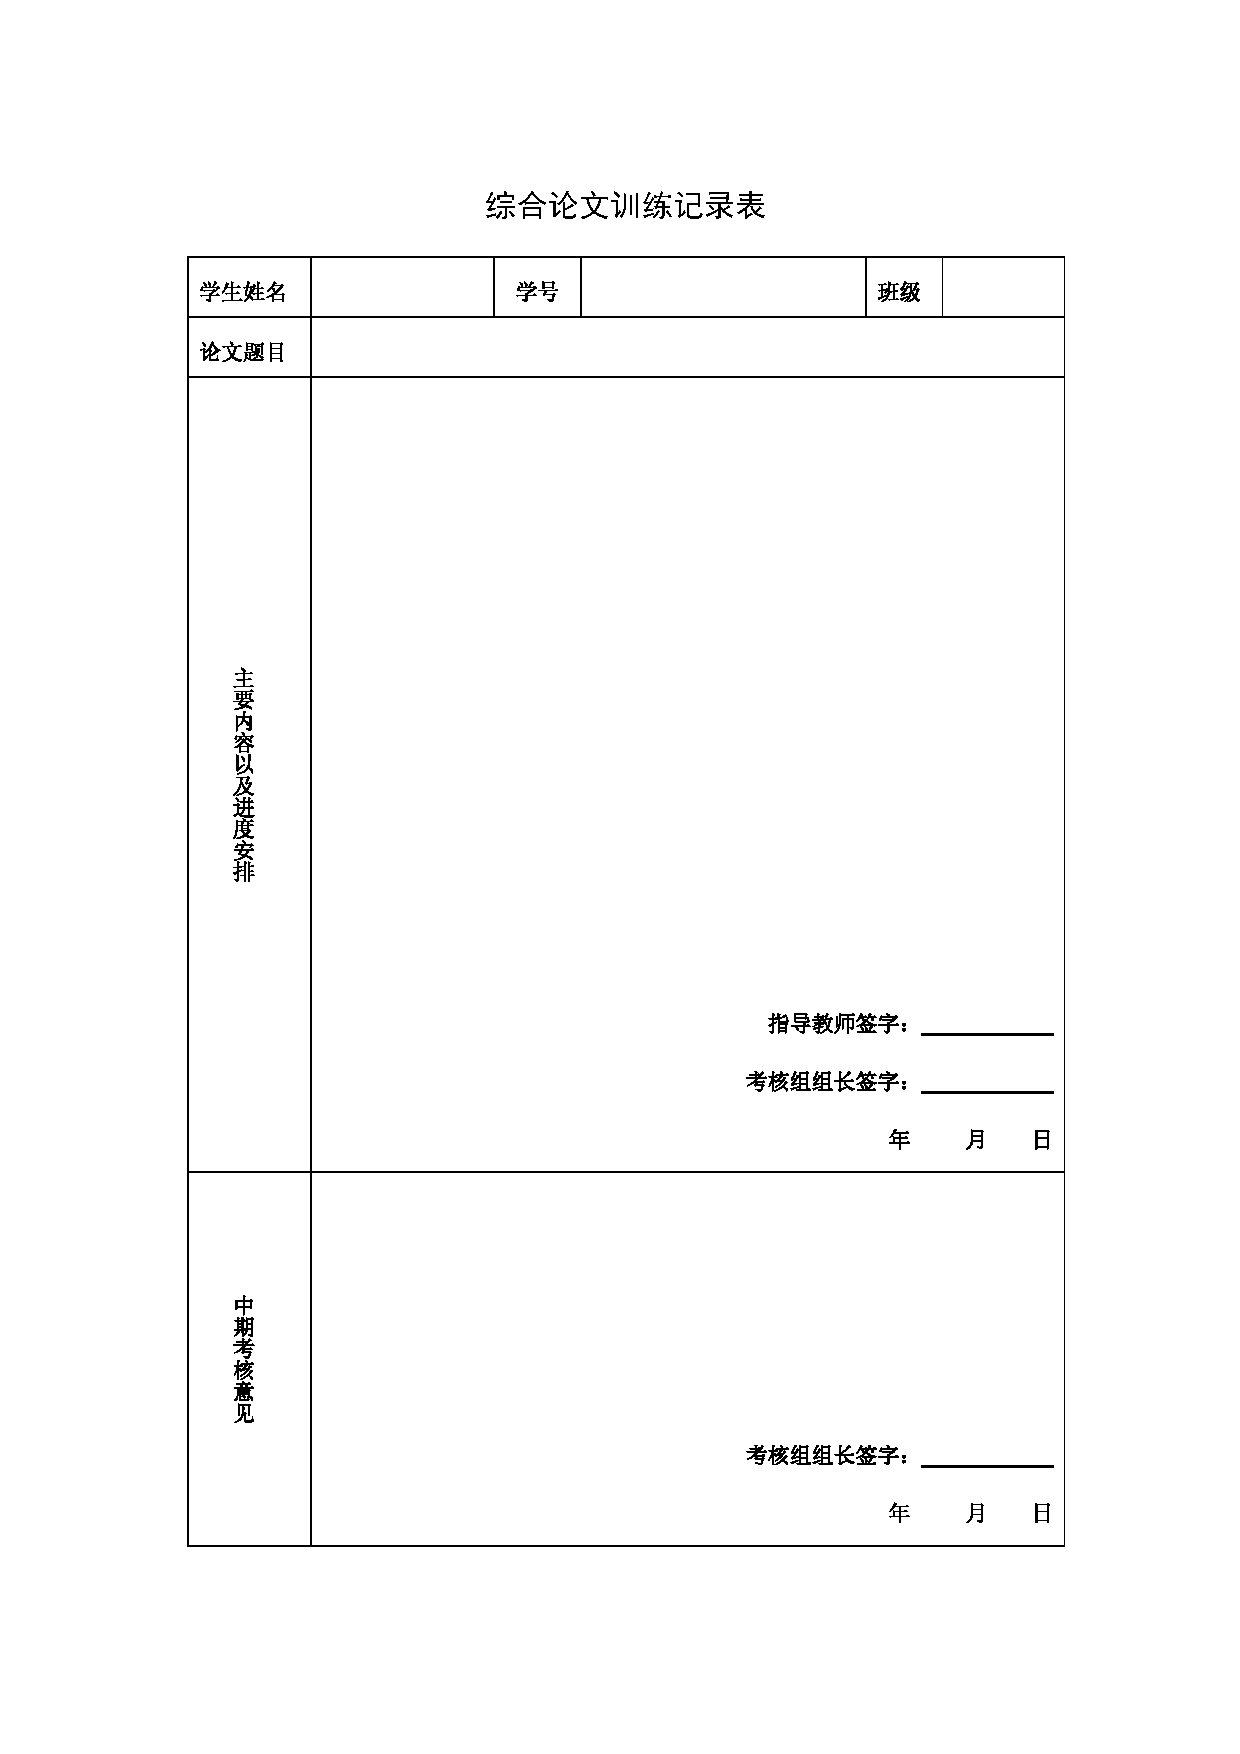
\includepdf[pages=-]{scan-record.pdf}
\end{document}
